\documentclass[border=3pt]{standalone}
\usepackage{tikz}
\usetikzlibrary{arrows.meta, positioning, fit, backgrounds}
\usepackage{amsmath}

\colorlet{strokeblue}{blue!70!cyan!80}
\colorlet{fillblue}{blue!70!cyan!4}
\colorlet{roadblockred}{red!75!black}
\colorlet{io green}{green!50!black}
\colorlet{greenok}{green!40!black}
\colorlet{redbad}{red!55!black}
\colorlet{orangewarn}{orange!70!black}

\begin{document}
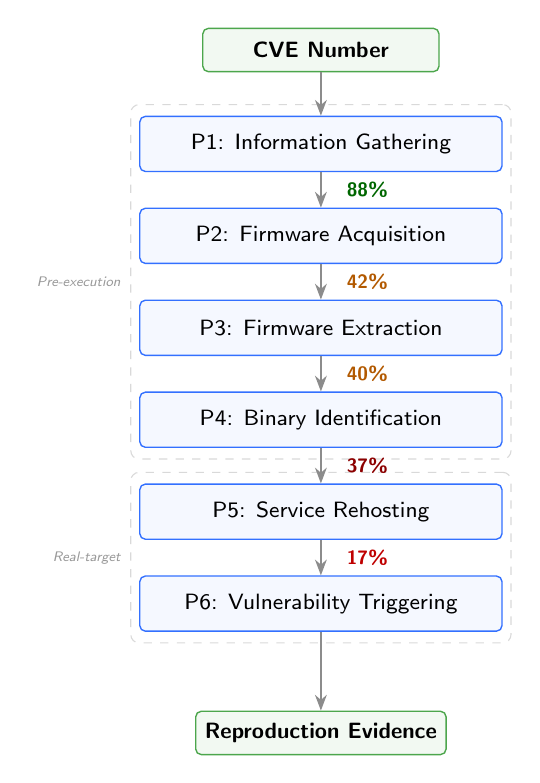
\begin{tikzpicture}[
    stage/.style={
        rectangle, rounded corners=2pt,
        minimum width=4.6cm, minimum height=0.7cm,
        text centered, draw=strokeblue, fill=fillblue,
        line width=0.5pt, font=\footnotesize\sffamily
    },
    arrow/.style={
        ->, line width=0.7pt, -{Stealth[length=2mm]},
        draw=black!45
    },
    io/.style={
        rectangle, rounded corners=2pt,
        minimum width=3cm, minimum height=0.55cm,
        text centered, draw=io green!70, fill=io green!5,
        line width=0.5pt, font=\footnotesize\sffamily\bfseries
    },
    rate/.style={
        font=\scriptsize\sffamily\bfseries, right=2mm
    },
    group/.style={
        draw=black!15, dashed, rounded corners=3pt,
        inner xsep=3pt, inner ysep=4pt
    },
    grouplabel/.style={
        font=\tiny\sffamily\itshape, text=black!40, anchor=east
    }
]

% ===== Nodes =====
\node[io] (in) {CVE Number};

\node[stage, below=0.55cm of in]      (s1) {P1: Information Gathering};
\node[stage, below=0.45cm of s1]      (s2) {P2: Firmware Acquisition};
\node[stage, below=0.45cm of s2]      (s3) {P3: Firmware Extraction};
\node[stage, below=0.45cm of s3]      (s4) {P4: Binary Identification};
\node[stage, below=0.45cm of s4]      (s5) {P5: Service Rehosting};
\node[stage, below=0.45cm of s5]      (s6) {P6: Vulnerability Triggering};

\node[io, below=1.0cm of s6]          (out) {Reproduction Evidence};

% ===== Arrows with reach rates (450 runs) =====
\draw[arrow] (in) -- (s1);
\draw[arrow] (s1) -- node[rate, text=greenok]    {88\%} (s2);
\draw[arrow] (s2) -- node[rate, text=orangewarn]  {42\%} (s3);
\draw[arrow] (s3) -- node[rate, text=orangewarn]  {40\%} (s4);
\draw[arrow] (s4) -- node[rate, text=redbad]      {37\%} (s5);
\draw[arrow] (s5) -- node[rate, text=roadblockred] {17\%} (s6);
\draw[arrow] (s6) -- (out);

% ===== Grouping boxes =====
\begin{scope}[on background layer]
    \node[group, fit=(s1)(s2)(s3)(s4)]  (gPre) {};
    \node[grouplabel] at (gPre.west) {Pre-execution};
    \node[group, fit=(s5)(s6)]                           (gExec) {};
    \node[grouplabel] at (gExec.west) {Real-target};
\end{scope}

\end{tikzpicture}
\end{document}
